\newif\ifglobal

%%%%%%%%%%%%%%%%%%%%%%%
%%% Compile to view %%%
%%%%%%%%%%%%%%%%%%%%%%%

%%%%%%%%%%%%%%%%%%%%%%%%%%%%%%%%%%%%%%%%%%%%%%%%%%%
%%% Readme:                                     %%%
%%% https://www.overleaf.com/read/bwdjvfjksvjy/ %%%
%%%%%%%%%%%%%%%%%%%%%%%%%%%%%%%%%%%%%%%%%%%%%%%%%%%

% >>> M?: marks a module setting number or important notice

% >>> M4: Set {./relative-path} to external files for this module <<<
\def \modulefiles {./58-TMPSEN}
% To add an external file, use:
% (Replace '---' with actual filename)
% '\input{\modulefiles/tables/---.tex}' for tables
% '\includegraphics{\modulefiles/figures/---}' for figures
% '\subfile{\modulefiles/---}' for register files

% >>> M1: This module is in global project? <<<
% 'YES' - uncomment; 'NO' - comment out
\globaltrue

\ifglobal
    \documentclass[main\_\_EN.tex]{subfiles}

\else
    \documentclass[openany, 10pt]{book}

    % >>> M2: In ./00-shared/preamble-trm-module, also find
    %         settings for visibility of todo notes, watermark <<<
    \usepackage{preamble-trm-module}

    % >>> M3: Temporary labels in English,
    %         you can add your own labels there <<<
    \myexternaldocument{./00-shared/temp-labels-en}

\fi %\ifglobal


\setcounter{secnumdepth}{4}


% >>> M5: If this module needs any updates in
% './00-shared/preamble-trm-module.sty'
% (include additional package, etc.), contact your module PM
% or create the file './00-shared/changelog.tex' make the
% necessary updates yourself and document them in this file <<<

% Make text left-aligned and allow latex to break pages naturally, comment out for full justification
\raggedright
\raggedbottom










\begin{document}


% Sets language into which pre-defined bits of text are translated
\selectlanguage{english}
\setenglishformatting

% Do not delete this block
\ifglobal
% Add the following front matter if
% this module is outside of global project
\else
    \InputIfFileExists{readme}{}{}
    \clearpage
    \listoftodos
    \listofdonetodos
    \tableofcontents
    %\listoftables
    %\listoffigures
\fi


%%%%%%%%%%%%%%%%%%%%%%%%%
%%% TRM Module Begins %%%
%%%%%%%%%%%%%%%%%%%%%%%%%

\hypertarget{tmpsen}{}
\chapter{Temperature Sensor}
\label{mod:tmpsen}


\section{Overview}

\chipname{} provides a temperature sensor to monitor temperature changes inside the chip in real time. The sensor converts analog voltage to digital values and supports compensation for the temperature offset.

\section{Features}
The temperature sensor has the following features:
\begin{itemize}
    \item Software-triggered temperature measurement. Once triggered, the sensor continuously measures temperature. Software can read the data any time.
    \item Hardware-triggered automatic temperature monitoring
    \item Two automatic temperature monitoring modes triggering interrupts upon threshold breaches
    \item Configurable temperature offset based on application scenarios to improve accuracy
    \item Configurable temperature measurement range
    \item Support for several Event Task Matrix (ETM) related events and tasks
\end{itemize}

\section{Architecture}

Figure \ref{fig:tsens_struct} shows the internal structure of the temperature sensor.
\begin{figure}[H]
    \centering
    \includegraphics[width=0.8\textwidth]{\modulefiles/figures/tsens_struct_20221209}
    \caption{Temperature Sensor Architecture}
    \label{fig:tsens_struct}
\end{figure}

As Figure \ref{fig:tsens_struct} shows, the temperature sensor module contains the following major blocks:

\begin{itemize}
    \item Tsens Ctrl \& Detect: controls temperature sensor sampling and checks the returned data
    \item HW Timer: periodically triggers temperature monitoring
    \item Tsens\_data Monitor: monitors whether the temperature is outside the threshold range
\end{itemize}

The temperature sensor operates as follows:
\begin{itemize}
    \item Enabling and initialization: The system configures the register via the APB bus to release Tsens\_pu\_apb. This signal is then synchronized to produce Tsens\_pu, which activates the temperature sensor's analog and digital circuits.
    \item Automatic hardware monitoring: When automatic monitoring is enabled, the HW Timer periodically generates the Monitor\_trigger signal at the configured sampling rate. This signal automatically triggers the Tsens Ctrl \& Detect module to perform a temperature conversion.
    \item Data comparison and evaluation: After each conversion, the 8-bit temperature data, Tsens\_data[7:0], is sent to the Tsens\_data Monitor. The monitor compares this data against the preset digital thresholds in real time.
    \item Interrupt and event output: When the temperature is outside of the preset threshold range, the monitor immediately outputs the raw over\_threshold signal. The synchronization module transfers this signal into the APB clock domain, generating the over\_threshold\_apb interrupt signal. This signal is then sent to the CPU or used to trigger an ETM event. Software can also obtain the current temperature value by reading \hyperref[fielddesc:TSENSOUT]{TSENS\_OUT}.
\end{itemize}


\section{Functional Description}

\subsection{Temperature Sensor Power Up}

The temperature sensor can be powered up by setting \hyperref[fielddesc:TSENSPOWERUP]{TSENS\_POWER\_UP}.

\subsection{Clock Management}

The temperature sensor clocks include:
\begin{itemize}
    \item Functional clock (FUNC\_CLK): two clock sources, RC\_FAST\_CLK and XTAL\_CLK
    \item Bus clock (BUS\_CLK): clock source is LPPERI\_SYS\_CLK
    \item Analog clock (ANA\_CLK): divided from the digital clock and configured by \hyperref[fielddesc:TSENSCLKDIV]{TSENS\_CLK\_DIV}
\end{itemize}

\begin{figure}[H]
     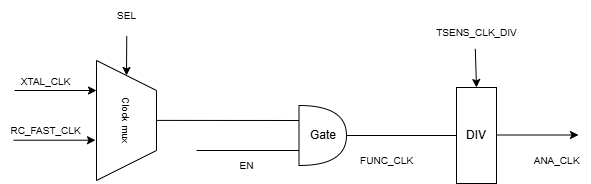
\includegraphics[width=0.8\linewidth]{58-TMPSEN/figures/TMPSENS_CLK_DIG.png}
     \centering
     \caption{\textcolor{black}{Temperature Sensor Clock Diagram}}
     \label{fig:tmpsen-clk}
 \end{figure}

As shown in Figure \ref{fig:tmpsen-clk}, the SEL signal comes from the system register \hyperref[fielddesc:FASTCLKSEL]{FAST\_CLK\_SEL}, and the EN signal comes from \hyperref[fielddesc:REGLPTSENSCLKEN]{LP\_TSENS\_CLK\_EN}. The analog clock is divided according to the following equation:
     \[
         f_{ANA\_CLK}=\frac{f_{FUNC\_CLK}}{TSENS\_CLK\_DIV+1}
     \]
 For more information on clocks, see Chapter \ref{mod:resclk} \textit{\nameref{mod:resclk}}.




 \subsection{Reset}

The temperature sensor has only one reset source:

\begin{itemize}
    \item Full reset: LP\_PERI\_RST\_BUS
\end{itemize}

\subsection{Automatic Temperature Monitoring Modes}

Two modes for the automatic temperature monitoring are available for selection by configuring \hyperref[fielddesc:TSENSWAKEUPMODE]{TSENS\_WAKEUP\_MODE}:

\begin{itemize}
    \item Absolute value mode:
        \begin{itemize}
            \item Monitors the absolute value of the current temperature. To set temperature thresholds, configure \hyperref[fielddesc:TSENSWAKEUPTHLOW]{TSENS\_WAKEUP\_TH\_LOW} and \hyperref[fielddesc:TSENSWAKEUPTHHIGH]{TSENS\_WAKEUP\_TH\_HIGH}. If the sampled value exceeds the high threshold or falls below the low threshold, an interrupt will be triggered.
        \end{itemize}
    \item Change value mode:
        \begin{itemize}
            \item Monitors the temperature changes inside the chip. If the temperature increment between two consecutive samplings exceeds the value configured in \hyperref[fielddesc:TSENSWAKEUPTHHIGH]{TSENS\_WAKEUP\_TH\_HIGH}, or the temperature decrement between two consecutive samplings exceeds the value configured in \hyperref[fielddesc:TSENSWAKEUPTHLOW]{TSENS\_WAKEUP\_TH\_LOW}, an interrupt will be triggered. For example, when \hyperref[fielddesc:TSENSWAKEUPTHLOW]{TSENS\_WAKEUP\_TH\_LOW} is configured to 8, if two consecutive sampling values are 28 and 19 respectively, i.e., the temperature decrement is 9, then an interrupt will be triggered.
        \end{itemize}
\end{itemize}

\subsection{Temperature Measurement Range and Offset}

To improve the temperature measurement accuracy, the temperature sensor is designed with five measurement ranges as shown in Table \ref{tab:tsensor-dac}. Each measurement range comes with specific measurement errors. Users do not need to worry about the errors, as they can choose specific offsets to get calibrated data.

\begin{longtable}[c]{|l|r|}
    \caption{Temperature Measurement Range and Offset}
    \label{tab:tsensor-dac}
    \\\hline
    \rowcolor{lightgray}
    Temperature Measurement Range (°C)   & Temperature Offset \\\hline
    50 \verb+~+ 125 & Determined by measured results \\\hline
    20 \verb+~+ 100 &  Determined by measured results \\\hline
    –10 \verb+~+ 80 &  Determined by measured results \\\hline
    –30 \verb+~+ 50 &  Determined by measured results \\\hline
    –40 \verb+~+ 20 &  Determined by measured results \\\hline
\end{longtable}

\subsection{Data Conversion}

The sensor output value is stored in \hyperref[fielddesc:TSENSOUT]{TSENS\_OUT}. To calculate the actual temperature \(T\) (°C) based on \(VALUE\), use the following equation:
\[
        T = 0.4386 * VALUE – 27.88 * offset – 20.52
\]

where \(offset\) is the temperature offset shown in Table \ref{tab:tsensor-dac}.


\section{Programming Procedure}

The temperature sensor can be started by software as follows:

\begin{enumerate}
    \item Set \hyperref[fielddesc:TSENSPOWERUP]{TSENS\_POWER\_UP} to power up the temperature sensor.
    \item Wait for \hyperref[fielddesc:TSENSXPDWAIT]{TSENS\_XPD\_WAIT} clock cycles till the temperature sensor releases from reset and starts measuring the chip temperature.
    \item Wait for 100 $\mu$s (so that the output value gradually approaches the actual temperature) and then read the data from \hyperref[fielddesc:TSENSOUT]{TSENS\_OUT}.
\end{enumerate}

To enable hardware-triggered automatic temperature monitoring, add the following programming steps before powering up the sensor:

\begin{enumerate}
    \item Configure \hyperref[fielddesc:TSENSSAMPLERATE]{TSENS\_SAMPLE\_RATE} to set sampling rate.
    \item Configure \hyperref[fielddesc:TSENSWAKEUPMODE]{TSENS\_WAKEUP\_MODE} to select an automatic temperature monitoring mode.
    \item Configure \hyperref[fielddesc:TSENSWAKEUPTHHIGH]{TSENS\_WAKEUP\_TH\_HIGH/LOW} to set the high and low temperature monitoring thresholds.
    \item Set \hyperref[fielddesc:TSENSWAKEUPEN]{TSENS\_WAKEUP\_EN} to start temperature monitoring.
    \item Configure \hyperref[fielddesc:TSENSWAKEUPMASK]{TSENS\_WAKEUP\_MASK} to 0 and \hyperref[fielddesc:TSENSCOCPUTSENSWAKEINTENA]{TSENS\_COCPU\_TSENS\_WAKE\_INT\_ENA} to 1 to enable interrupt reporting.
    \item Set \hyperref[fielddesc:TSENSSAMPLEEN]{TSENS\_SAMPLE\_EN} to enable automatic temperature monitoring.
\end{enumerate}

In automatic temperature monitoring mode, the output value will not be stored. However, users can get the value anytime from \hyperref[fielddesc:TSENSOUT]{TSENS\_OUT}.

\section{Interrupts}

\chipname{}'s Temperature Sensor can generate the following interrupt signal that will be sent to the \hyperref[mod:intmtrx]{Interrupt Matrix}.

\begin{itemize}
    \item LP\_TSENS\_INTR
\end{itemize}

There is one internal interrupt source from the temperature sensor that can generate the above interrupt signal:

\begin{itemize}
    \item \label{interrupt:TSENSCOCPUTSENSWAKEINT} TSENS\_COCPU\_TSENS\_WAKE\_INT: Triggered when the condition of the mode selected by \hyperref[fielddesc:TSENSWAKEUPMODE]{TSENS\_WAKEUP\_MODE} is met.
    \begin{itemize}
        \item Absolute value mode: the sampled value is above \hyperref[fielddesc:TSENSWAKEUPTHHIGH]{TSENS\_WAKEUP\_TH\_HIGH} or below \hyperref[fielddesc:TSENSWAKEUPTHLOW]{TSENS\_WAKEUP\_TH\_LOW}.
        \item Change value mode: the increment between two consecutive samples exceeds \hyperref[fielddesc:TSENSWAKEUPTHHIGH]{TSENS\_WAKEUP\_TH\_HIGH}, or the decrement exceeds \hyperref[fielddesc:TSENSWAKEUPTHLOW]{TSENS\_WAKEUP\_TH\_LOW}.
    \end{itemize}
\end{itemize}

\begin{tiplisting}
For definitions of \textit{interrupt}, \textit{interrupt signal}, \textit{interrupt source}, and their correlations, please refer to Chapter \ref{mod:intmtrx} \textit{\nameref{mod:intmtrx}} > Section \ref{sec:intmtx-int-terminology} \textit{\nameref{sec:intmtx-int-terminology}}.
\end{tiplisting}

Each interrupt source can be configured by a common set of registers that are described in Section \hyperref[interrupt-config-registers]{\textit{Interrupt Configuration Registers}}. The specific registers can be found in Section \ref{sec:tmpsen-reg-summ} \textit{\nameref{sec:tmpsen-reg-summ}}.

%%%%%%%%%%%%%%%%%%%%%%%%%%%%%%%%%
%%% Event Task Matrix Feature %%%
%%%%%%%%%%%%%%%%%%%%%%%%%%%%%%%%%

\section{Event Task Matrix Feature}
\label{sec:tmpsen-etm-func}

The temperature sensor on \chipname{} supports the Event Task Matrix (ETM) function, which allows the temperature sensor's ETM tasks to be triggered by any peripherals' ETM events, or temperature sensor's ETM events to trigger any peripherals' ETM tasks. This section introduces the ETM tasks and events related to the temperature sensor. For more information, please refer to Chapter \ref{mod:evntaskmatrix} \textit{\nameref{mod:evntaskmatrix}}.
The temperature sensor can receive the following ETM tasks:

\begin{itemize}
    \item TMPSNSR\_TASK\_START\_SAMPLE: The temperature sensor starts sampling when this task is triggered.
    \item TMPSNSR\_TASK\_STOP\_SAMPLE: The temperature sensor stops sampling when this task is triggered.
\end{itemize}

The temperature sensor can generate the following ETM events:

\begin{itemize}
    \item TMPSNSR\_EVT\_OVER\_LIMIT: Generated when the temperature is beyond the threshold.
\end{itemize}

In practical applications, temperature sensor's ETM events can trigger its own ETM tasks. For example, the TMPSNSR\_EVT\_OVER\_LIMIT event can trigger the TMPSNSR\_TASK\_STOP\_SAMPLE task.

% >>> If your module has no registers, delete sample text
%       for Sections Register Summary and Registers below <<<

%%%%%%%%%%%%%%%%%%%%%%%%
%%% Register Summary %%%
%%%%%%%%%%%%%%%%%%%%%%%%

% >>> Update the sample text below and insert
%     the info on register summary into the subfile <<<

\newpage
\hypertarget{tmpsen-reg-summ}{}
\section{Register Summary}
\label{sec:tmpsen-reg-summ}

The addresses in this section are relative to Temperature Sensor base address provided in Table \ref{tab:sysmem-base-address} in Chapter \ref{mod:sysmem} \textit{\nameref{mod:sysmem}}.

The abbreviations given in Column \textbf{Access} are explained in Section \hyperref[glossary-access-types]{\textit{Access Types for Registers}}.
\subfile{\modulefiles/58-TMPSEN-reg-summ__EN}

%%%%%%%%%%%%%%%%%
%%% Registers %%%
%%%%%%%%%%%%%%%%%

% >>> Update the sample text below and insert
%      the info on registers into the subfile <<<

\newpage
\section{Registers}

The addresses in this section are relative to Temperature Sensor base address provided in Table \ref{tab:sysmem-base-address} in Chapter \ref{mod:sysmem} \textit{\nameref{mod:sysmem}}.

For how to program reserved fields, please refer to Section \hyperref[programming-reserved-field]{\textit{Programming Reserved Register Field}}.

\subfile{\modulefiles/58-TMPSEN-reg__EN}

\end{document}
